% ****** Start of file apssamp.tex ******
%
%   This file is part of the APS files in the REVTeX 4.1 distribution.
%   Version 4.1r of REVTeX, August 2010
%
%   Copyright (c) 2009, 2010 The American Physical Society.
%
%   See the REVTeX 4 README file for restrictions and more information.
%
% TeX'ing this file requires that you have AMS-LaTeX 2.0 installed
% as well as the rest of the prerequisites for REVTeX 4.1
%
% See the REVTeX 4 README file
% It also requires running BibTeX. The commands are as follows:
%
%  1)  latex apssamp.tex
%  2)  bibtex apssamp
%  3)  latex apssamp.tex
%  4)  latex apssamp.tex1khz
%
\PassOptionsToPackage{english}{babel}
\documentclass[aps,prl,
reprint,
superscriptaddress,
%groupedaddress,
%unsortedaddress,
%runinaddress,
%frontmatterverbose, 
%preprint,
%onecolumn, %%
%preprintnumbers,
%nofootinbib,
%nobibnotes,
%bibnotes,
 amsmath,amssymb,
%pra,
%prb,
%rmp,
%prstab,
%prstper,
floatfix
]{revtex4-2}
\usepackage[dvipsnames]{xcolor}
\usepackage{graphicx}% Include figure files
\usepackage{dcolumn}% Align table columns on decimal point
\usepackage{bm}% bold math
\usepackage{outlines}
\usepackage{float}
\usepackage{textcomp}
\usepackage{hyperref}
\usepackage{subfigure}
\let\vec=\mathbf

\usepackage{titlesec}
% \titleformat*{\section}{\centering\large\bfseries}
% \titleformat*{\subsection}{\normalfont\centering}
% \titlespacing{\section}{0pt}{3pt}{3pt}
% \titlespacing{\subsection}{0}{3pt}{3pt}

\usepackage[normalem]{ulem}

\usepackage{braket}
\newcommand{\derivn}[3][{}]{
    \frac{d^{#1} #2}{d #3^{#1}}
}

\newcommand{\MetastableState}{2^{3\!}S_1}%
\newcommand{\UpperStates}{3^{3\!}P_{0,1,2}}%
\newcommand{\UpperStateManifold}{3^{3\!}P}%
\newcommand{\LowerStates}{2^{3\!}P_{(0,1,2)}}%
\newcommand{\LowerStateManifold}{2^{3\!}P}%
\newcommand{\GroundState}{1^{1\!}S_{0}}%
\newcommand{\SingletState}{2^{1\!}S_0}%
\newcommand{\TO}{\MetastableState- \LowerStateManifold / \UpperStateManifold}%
\newcommand{\polz}{\alpha(f)}% \operatorname{Re}()  , cand have real part implicit

\newcommand{\brycerev}[1]{{\color{Purple}{#1}\normalcolor}} %revision from Bryce
\newcommand{\brycecom}[1]{{\color{ProcessBlue}[BMH:{#1}]\normalcolor}} %Comments from Bryce
\newcommand{\andrewcom}[1]{{\color{Orange}[AGT:{#1}]\normalcolor}}
\newcommand{\theoryq}[1]{{\color{Green}[Theory Question:{#1}]\normalcolor}}
\newcommand{\todocom}[1]{{\color{Red}[TODO:{#1}]\normalcolor}} 


\usepackage{textcomp}


\begin{document}

\title{
Precision Measurement of the Helium $\TO$ Tune-Out Frequency as a Test of QED
}



\author{B. M. Henson}
\thanks{These authors contributed equally}
\affiliation{Laser Physics Centre, Research School of Physics, The Australian National University,\\ Canberra, ACT 2601, Australia}

\author{J. A. Ross}
\thanks{These authors contributed equally}
\affiliation{Laser Physics Centre, Research School of Physics, The Australian National University,\\ Canberra, ACT 2601, Australia}

\author{K. F. Thomas}
\affiliation{Laser Physics Centre, Research School of Physics, The Australian National University,\\ Canberra, ACT 2601, Australia}

\author{C. N. Kuhn}
\affiliation{Center for Quantum and Optical Science, Swinburne University of Technology, Melbourne, Australia}

\author{D. K. Shin}
\affiliation{Laser Physics Centre, Research School of Physics, The Australian National University,\\ Canberra, ACT 2601, Australia}

\author{S. S. Hodgman}
\affiliation{Laser Physics Centre, Research School of Physics, The Australian National University,\\ Canberra, ACT 2601, Australia}

\author{Yong-Hui Zhang}
\affiliation{State Key Laboratory of Magnetic Resonance and Atomic and Molecular Physics, Innovation Academy for Precision Measurement Science and Technology, Chinese Academy of Sciences, Wuhan 430071, People's Republic of China}

\author{Li-Yan Tang}
\email{lytang@wipm.ac.cn}
\affiliation{State Key Laboratory of Magnetic Resonance and Atomic and Molecular Physics, Innovation Academy for Precision Measurement Science and Technology, Chinese Academy of Sciences, Wuhan 430071, People's Republic of China}

\author{G. W. F. Drake}
\email{gdrake@uwindsor.ca}
\affiliation{Physics Department, University of Windsor, Windsor, Ontario, Canada}

\author{A. T. Bondy}
\affiliation{Physics Department, University of Windsor, Windsor, Ontario, Canada}

\author{A. G. Truscott}
\email{andrew.truscott@anu.edu.au}
\affiliation{Laser Physics Centre, Research School of Physics, The Australian National University,\\ Canberra, ACT 2601, Australia}

\author{K. G. H. Baldwin}
\email{kenneth.baldwin@anu.edu.au}
\affiliation{Laser Physics Centre, Research School of Physics, The Australian National University,\\ Canberra, ACT 2601, Australia}

\date{\today}

%TO DO
%%%%%%%%%%%%%%%%%%%%%%%%%%%%%%%%%%%%%%%%%%%%%%%%%%%%%%%
% feedback by author, x marks completion of feedback and that the author has agreed to the manuscript being submitted for publication

% [ ] B M Henson
% [x] J A Ross
% [x] K F Thomas
% [x] C N Kuhn
% If I understood correct the laser was scanned the frequency instead to be jumping randomly  between frequencies during the tune-out measurement, how do you count for possible drifts during the data collection? If the data was collected randomly I missed this out from the draft.

% [x] D K Shin
% [x] S S Hodgman
% [x] Y H Zhang
% [x] L Y Tang
% [ ] G W F Drake
% derivatives

% [x] A T Bondy
% [x] A G Truscott
% [x] K G H Baldwin


%%%%%%%%%%%%%%%%%%%%%%%%%%%%%%%%%%%%%%%%%%%%%%%%%%%%%%%
\begin{abstract}
Despite quantum electrodynamics (QED) being one of the most stringently tested theories underpinning modern physics, recent precision atomic spectroscopy measurements have uncovered several small discrepancies between experiment and theory.  One particularly powerful experimental observable that tests QED independently of traditional energy level measurements is the `tune-out' frequency, where the dynamic polarizability vanishes and the atom does not interact with applied laser light.  In this work, we measure the `tune-out' frequency for the \(\MetastableState\) state of helium between transitions to the $\LowerStateManifold$ and $\UpperStateManifold$ manifolds and compare it to new theoretical QED calculations.  The experimentally determined value of 725\,736\,700\,$(40_{\mathrm{stat}},260_{\mathrm{syst}})$~MHz is within \({\sim} 2.5\sigma\) of theory (725\,736\,053(9)~MHz), and importantly resolves both the QED contributions (\({\sim} 30 \sigma\)) and novel retardation (\({\sim} 2 \sigma\)) corrections.
\end{abstract}
%725\,736\,480

% Laser light can be made invisible to an atom by precisely tuning to a frequency between transitions at which the dynamic polarizability vanishes.
% We measure this `tune-out' frequency for the  $\MetastableState$ state of helium between transitions to the $\LowerStateManifold$ and $\UpperStateManifold$ manifolds to test quantum electrodynamics (QED) independently of traditional energy level measurements.
% We also present a new theoretical estimate for the tune-out frequency.
% The new experimental determination of 725\,736\,700\,$(40_{\mathrm{stat}},260_{\mathrm{syst}})$~MHz represents a twenty-fold improvement in precision over the first experimental measurement and
% lies around \(+0.8\sigma\) from our new theoretical prediction of 725\,736\,480\,(6)~MHz. Importantly, we are able to resolve the QED contributions (\({\sim} 30 \sigma\)) and retardation corrections (\({\sim} 2 \sigma\)) to the tune-out frequency.

\maketitle
% 2500 words max for science !!!!!

Quantum electrodynamics (QED) describes the interaction between matter and light. It is so ubiquitous that the theory is considered a cornerstone of modern physics.
QED has been remarkably predictive in describing fundamental processes, such as spontaneous emission rates of photons from atoms and the anomalous electron magnetic moment \cite{PhysRevD.91.033006}.
However, as the precision of atomic spectroscopy approaches the part-per-trillion level, discrepancies between such predictions and experiments have come to light, such as the `proton radius puzzle'. Spectroscopic measurements (of $\mu+p$ \cite{Pohl2010}, H \cite{Bezginov1007,Beyer79}, and $\mu +2p$ \cite{Pohl669}) yield determinations of the proton radius which disagree by up to five standard deviations with other approaches (e+p scattering \cite{ZHAN201159}, and H spectroscopy\cite{PhysRevLett.120.183001}). 


Helium is an exemplary testing ground for QED because its simple two-electron structure makes high-precision predictions tractable and testable. Notably helium also presents a nuclear `puzzle', with precision measurement of isotope shifts of the \(\MetastableState \rightarrow \LowerStates \) \cite{PhysRevLett.119.263002} and \(\MetastableState \rightarrow \SingletState \) \cite{Rengelink2018} transitions disagreeing at two standard deviations in the derived nuclear charge radius. These `puzzles' raise the possibility that the issue lies with QED itself \cite{refId0}. Thus, we look to challenge QED directly by precision spectroscopy in helium beyond the usual energy interval measurements.


An atom in an optical field experiences an energy shift in proportion to the real part of the frequency dependent polarizability, a fundamental atomic property dictated by the position of energy levels and the strengths of transitions to them (Fig. \ref{fig:schematic}). 
A ‘tune-out’ frequency ($f_\mathrm{TO}$) occurs between transition frequencies at the point where the contributions to the dynamic polarizability [$\alpha(f)$] by all transitions below that frequency are balanced by all those above it ($\alpha(f)=0$) \cite{PhysRevA.75.053612}. 
This balance point is hence fixed by the strength and frequency of every transition in the atomic spectrum and thus provides a precise constraint on the ratio of transition dipole matrix elements. 

%background work and previous tune-out measurements
As a test of QED, a tune-out frequency is advantageous because it is a null measurement, which does not require calibration of the light intensity or a measurement of excitation probability. These factors have previously limited the precision of direct transition strength measurements \cite{Bouloufa_2009,Vogt2007,PhysRevLett.125.013002}. In comparison, previous tune-out measurements have been successful in measuring QED effects \cite{PhysRevA.92.052501,PhysRevLett.109.243004,PhysRevA.93.022507,PhysRevLett.109.243003,PhysRevLett.115.043004}.
%Previous approaches to measuring the small potentials produced by a laser beam tuned near a tune-out frequency include atom interferometry \cite{PhysRevA.92.052501,PhysRevLett.109.243004}, motional scattering in an optical lattice \cite{PhysRevA.93.022507,PhysRevLett.109.243003} and atom-laser dynamics \cite{PhysRevLett.115.043004}. 

%our experimental work
In this work we measure the tune-out of the metastable $\MetastableState$ state of helium (denoted He*) which lies between transitions to the $\LowerStateManifold$ and $\UpperStateManifold$ manifolds (denoted $\TO$) at approximately 726~THz (413~nm). We chose this particular tune-out frequency as the two neighbouring transitions are more than an octave apart in frequency, causing the gradient of atomic polarizability with optical frequency to be very small at the tune-out. Hence, this tune-out frequency is especially sensitive to higher order QED effects. We achieve a 20-fold improvement in the precision over the sole previous measurement \cite{PhysRevLett.115.043004}.
\begin{figure} 
\centering
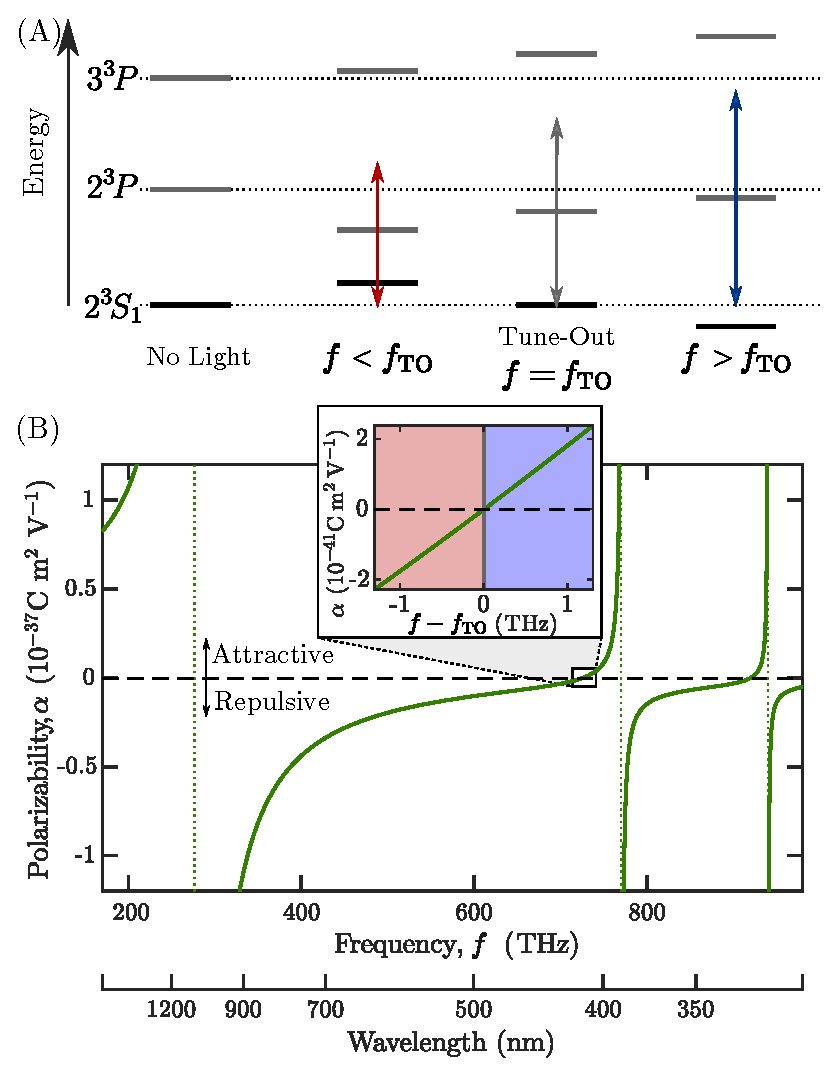
\includegraphics[width=0.48\textwidth]{figs/composite_polz_fig}
\caption{\textbf{Tune-out in atomic helium:}
(A) Atomic energy level shift of the dominant state (manifolds) about the tune-out.  When an optical field of frequency $f$ (arrows) is applied to the atom the individual
levels shift dependent on the difference between $f$ and the transition frequency. At the tune-out frequency $f_{\mathrm{TO}}$ (middle right), the shifts to the $\MetastableState$ state energy cancel.
Energy spacing and shifts not to scale.
(B) Theoretical frequency dependent polarizability of $\MetastableState$ helium, for a constant light polarisation, indicating that the polarizability vanishes near 726~THz, - the tune-out frequency measured in this paper. 
Vertical dotted lines show, from left to right, the transitions to the  $\LowerStateManifold$, $\UpperStateManifold$,$4^{3\!}P$ manifolds. Inset shows the approximately linear polarizability with frequency about the tune-out.
}
\label{fig:schematic} 
\end{figure}

\begin{figure*}[t]
\centering
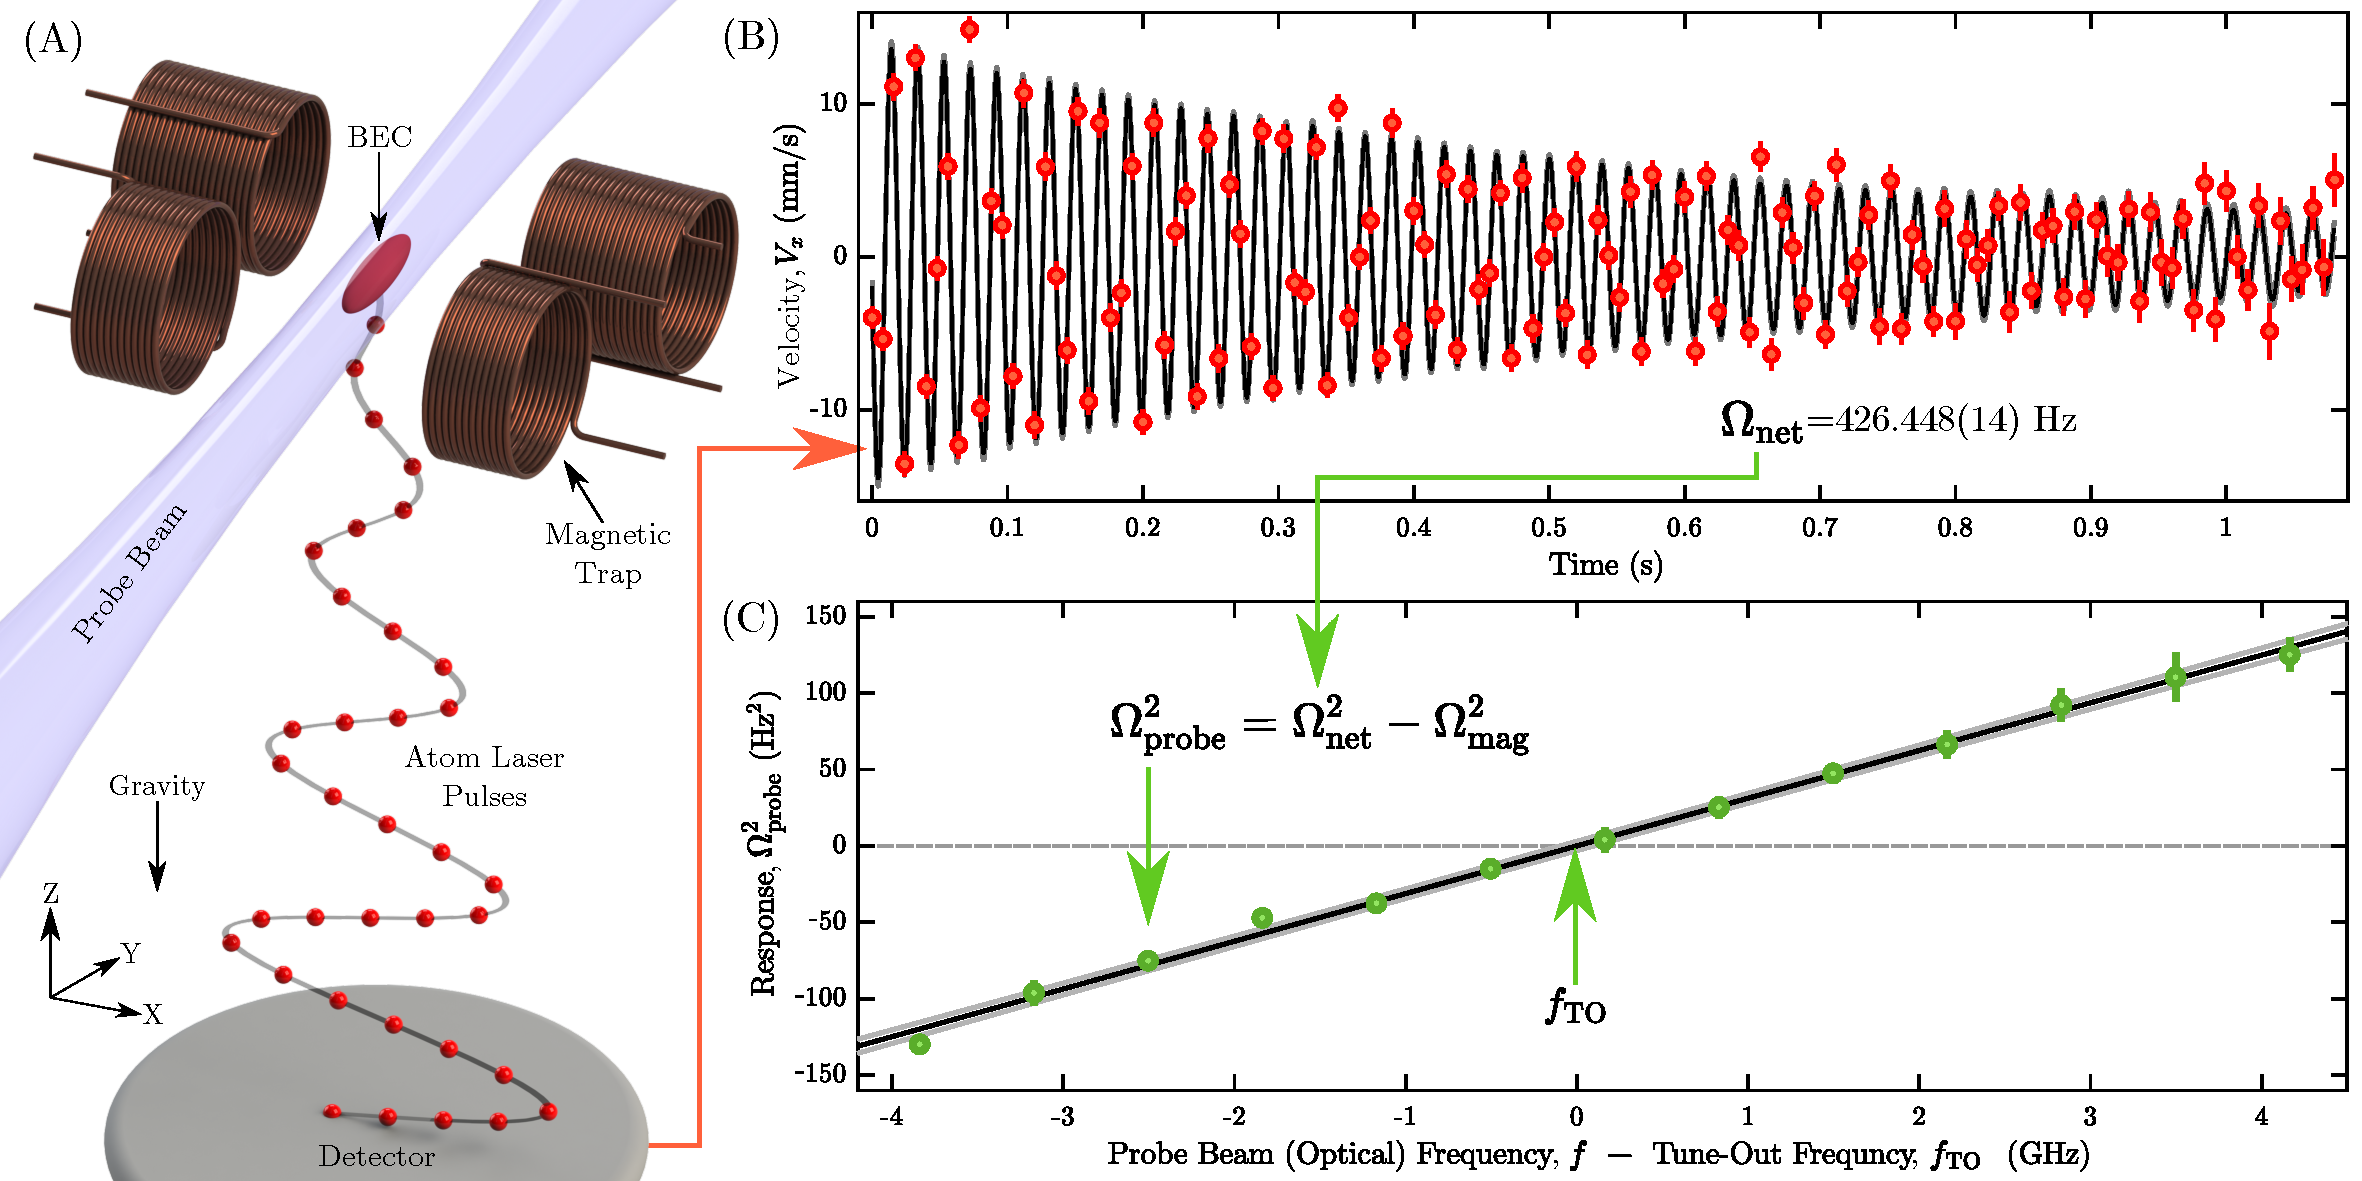
\includegraphics[width=1\textwidth]{figs/method_stage1and2_processing_schematic_v4.pdf}
\caption{
\textbf{Experimental procedure:} Method to determine the tune-out for a fixed probe beam polarization. (A) a magnetically trapped BEC of metastable helium atoms is illuminated with a probe laser beam with an adjustable (optical) frequency. A sequence of atom laser pulses is outcoupled from the BEC to sample the oscillation. (B) The mean velocity of each pulse in the \textit{x}-direction ($v_x$) is used to trace out the oscillation over time (red points) and extract the oscillation frequency with a dampened sine wave fit (solid line). A single experimental realization is shown. (C) The squared probe beam trap frequency (response) is found using a separate measurement of the magnetic trap frequency. This measurement is repeated over a small range of optical frequencies. The tune-out is extracted by finding the \textit{x}-intercept of the response as a function of probe beam frequency using a linear fit (black solid line). Light grey lines show the model \(1\sigma\) confidence intervals. All error bars represent the standard error in the mean.
}
\label{fig:stage_1_processing_schematic} 
\end{figure*}


%theory work
For an unambiguous comparison we also present a new theoretical estimate of the \(\TO\) tune-out in helium. Following the first prediction \cite{PhysRevA.88.052515} and measurement \cite{PhysRevLett.115.043004} of the tune-out, a vigorous campaign of theoretical studies \cite{PhysRevA.93.052516,manalo2017variational,Drake2019,PhysRevA.99.040502, PhysRevA.99.041803} has reduced the uncertainty in the predicted frequency, which limited comparison with experiment. Our work represents a 10-fold improvement in precision over previous calculations, and whose uncertainty now surpasses the experimental state-of-the-art.


Measuring a tune-out frequency amounts to measuring the potential energy of a light field interacting with an atom, known as an optical dipole potential \cite{grimmOpticalDipoleTraps2000}, and identifying precisely the frequency at which it vanishes (see Fig.~\ref{fig:schematic}). The new experimental approach taken here measures the optical dipole potential via changes in the spatial oscillation frequency (also called trap frequency) of Bose-Einsten condensates (BECs) in a harmonic magnetic trap when overlapped with a laser probe beam (see Fig.~\ref{fig:stage_1_processing_schematic}). The net potential energy is the sum of a harmonic magnetic potential and a Gaussian optical potential, which is approximately harmonic for the small oscillation amplitudes we consider. In this limit the oscillation frequency is given by $\Omega_{\text{net}}^2=\Omega_{\text{mag}}^2+\Omega_{\text{probe}}^2$ where \(\Omega_{\text{mag}}\), \(\Omega_{\text{probe}}\), and \(\Omega_{\text{net}}\) denote the trap frequency of the magnetic, probe, and combined potentials respectively. For a Gaussian beam profile, as used here, the probe perturbation scales as \(\Omega_{\text{probe}}^2\propto \alpha(f) I\), where I is the intensity of the probe beam. Hence, with the probe beam power stabilized, the difference of squared trapping frequencies \(\Omega_{\text{net}}^2-\Omega_{\text{mag}}^2\propto\alpha(f)\) produces a response which is linearly proportional to the dynamic polarizability. Having measured the transverse and longitudinal profiles of the probe beam, the shift in trapping frequency completely specifies the optical dipole potential. 
%and permits us to discern a peak potential energy of as little as 10$^{-35}$J. This is, to our knowledge, the smallest precision in a potential energy measurement reported to date \cite{SOMs}.  


We determine the trap frequency of our BECs with a novel method which repeatedly samples the momentum of an oscillating BEC with a \textit{pulsed atom laser} \cite{PhysRevLett.78.582,Manning:10} (Fig.~\ref{fig:stage_1_processing_schematic}(A)). Each measurement starts by generating a new He* BEC, which is set in motion by applying a field gradient, and is then depleted over the course of the trap frequency measurement (1.2~s long, see Fig.~\ref{fig:stage_1_processing_schematic}(B)). The starting sample of atoms is cooled to ${\sim}80$~nK, well below the critical temperature, to reduce the damping that ultimately limits the interrogation time and, in turn, uncertainty in the trapping frequency. We alternate between measurements of trapping frequency with and without the optical potential to calibrate for any long term drift in \(\Omega_{\text{mag}}\). We then measure the change in (squared) trap frequency due to the probe beam, \(\Omega_{\text{probe}}^2\), as a function of the probe beam (optical) frequency $f$ near the tune-out frequency at  ${\sim} 726$~THz (413~nm). The small laser frequency scan range used in our experiment allows us to determine the tune-out frequency \(f_{\text{TO}}\) via linear interpolation from the measured response of $\Omega_{\text{probe}}^2$ (Fig.~\ref{fig:stage_1_processing_schematic}(C)).

The dynamic atomic polarizability consists of the frequency dependent scalar, vector, and tensor components (\(\alpha^S(f),\alpha^V(f),\alpha^T(f)\) respectively). The total polarizability (and hence the tune-out) also depends on the degree of linear and circular polarization in the atom's reference frame, given by the second and fourth Stokes parameters \(\mathcal{Q_{A}}\) and  \(\mathcal{V}\) respectively, and on the angle $\theta_k$ between the laser propagation direction and the magnetic field vector \cite{LeKien2013}. The tune-out frequency for the \(\MetastableState\) state and arbitrary polarization is: 

\begin{widetext}
    \begin{equation}
    f_{\mathrm{TO}}(\mathcal{Q_{A}}, \mathcal{V}) = f^{S}_{\mathrm{TO}} + \frac{1}{2} \beta^V \cos \left( \theta_k \right) \mathcal{V}  - \frac{1}{2} \beta^T \left[3 \sin^2\left( \theta_k \right) \left(\frac{1}{2} +  \frac{\mathcal{Q_{A}(Q_{L},\theta_{L}})}{2}\right) -1 \right],
    \label{eq:TO_model}
    \end{equation}
\end{widetext}
where \(f^{S}_{\mathrm{TO}}\) is the tune-out frequency for the scalar polarizability $\alpha^S(f)$, \(\mathcal{Q_{A}(Q_{L},\theta_{L}})\) is the second Stokes parameter in terms of the laboratory measurement of the second Stokes parameter \(\mathcal{Q_L}\), and the angle between the lab and atomic frames \(\mathcal{\theta_{L}}\). Here, \( \beta^V\) and  \(\beta^T\) are the vector and tensor polarizabilities divided by the gradient of the scalar polarizability (with respect to frequency) at the tune-out \cite{SOMs}.


We measure the tune-out \(f_{\mathrm{TO}}(-1,0)\), corresponding to a linearly polarised light-field whose polarisation axis is perpendicular to both the laser propagation and the magnetic field. For this configuration, the sensitivity to \(\theta_{k}\) and \(\theta_\mathcal{L}\) is minimized and the atomic polarizability simplifies to

\begin{equation}
    \alpha(f) = \alpha^S(f) - \frac{1}{2} \alpha^T(f). 
    \label{eq:polarizability_2}
\end{equation}

We measure \(f_{\mathrm{TO}}(\mathcal{Q_{A}}, \mathcal{V}) \) as a function of the probe beam polarization parameters \(\mathcal{Q_{A}}\) and \(\mathcal{V}\) and interpolate using Eq.~(\ref{eq:TO_model}) to determine \(f_{\mathrm{TO}}(-1,0)\) (see Fig.~\ref{fig:pol_TO}). We take the sign of \(\beta^T\) from theory, but use no other predictions in our calculation. Thus, we determine a value of  725\,736\,700\,$(40_{\mathrm{stat}},260_{\mathrm{syst}})$ MHz for the \(f_{\mathrm{TO}}(-1,0)\) tune-out, including systematic effects \cite{SOMs}.


\begin{figure}
\centering

\includegraphics[width=0.47\textwidth]{figs/to_q_crop.png}
\includegraphics[width=0.47\textwidth]{figs/to_v_crop.png}
\caption{\textbf{Tune-out dependence on probe beam polarisation:}
(A) Dependence of the measured tune-out on $\mathcal{Q_{A}}$ when interpolated to $\mathcal{V}=0$. (B) Dependence of the measured tune-out on $\mathcal{V}$ when interpolated to $\mathcal{Q_{A}}=-1$. The linear fits are both of the form of Eq.~(\ref{eq:TO_model}), with fit parameters \(f_{TO}(-1,0)=725\,736\,700\,(40)\)~MHz, \(\beta^V \cos(\theta_k)=13\,240\,(70)\)~MHz, \(\beta^T \sin^2(\theta_k)=1\,140\,(20)\)~MHz (uncertainties represent only statistical uncertainty; see Ref.~\cite{SOMs} for full error budget). Error bars show the estimated standard error.
} 
\label{fig:pol_TO} 
\end{figure}


The dominant systematic effect in our measurement is the uncertainty in the light polarization. The probe beam passes through a vacuum window before it interacts with the atoms, which may subtly alter the laser polarization relative to measurements made outside the vacuum chamber.
We constrain this error to be less than 200~MHz by measuring the probe beam polarization before entering, and after exiting, the vacuum system \cite{SOMs}. 
%We hence bound this uncertainty to be less than 200~MHz. 


Separately, we improve on the state-of-the-art calculation \cite{PhysRevA.99.040502} of the tune-out frequency by accounting for finite nuclear mass, relativistic, QED, finite nuclear size, negative energy states, and finite wavelength retardation effects \cite{Drake2019, PhysRevA.99.041803,SOMs}. 
We achieve a 10-fold improvement in precision and find a theoretical value of \(725\,736\,053(9)\)~MHz for \(f_{\mathrm{TO}}(-1,0)\). The major contribution to the theoretical uncertainty stems from the QED contribution (\(\pm 8\)~MHz), which is an order of magnitude less than the systematic experimental uncertainty.
We show a comparison of our experimental and theoretical uncertainties to the main contributions of interest to the theoretical value in Fig.~\ref{fig:contributions}, to demonstrate the contributions to which our measurement is sensitive.


\begin{figure}[t]
    \centering
    \includegraphics[width=0.48\textwidth]{figs/contribution_bar_chart_v7.png}
    \caption{\textbf{Experimental and theoretical sensitivity:} Comparison of uncertainties in the theoretical and experimental determinations of the \(\TO\) tune-out frequency and the various theoretical contributions to the tune-out value.}
    \label{fig:contributions}
\end{figure}


 To summarise, our experimental determination of 725\,736\,700\,$(40_{\mathrm{stat}},260_{\mathrm{syst}})$ MHz is a \(20\)-fold improvement over the first experimental determination, and is 2.5$\sigma$ larger than the theoretical prediction. Our measurement corresponds to a relative precision in oscillator strength ratio of 6 ppm \cite{SOMs}, which is a factor of two improvement on the previous record \cite{PhysRevA.88.052515}. The combined theoretical and experimental uncertainties (\({\sim} 260\)~MHz) are able to discern the contribution of QED effects (\({\sim} 30 \sigma\)), and are similar to the retardation corrections to the dipole interaction (\({\sim} 2 \sigma\)), but much greater than the contribution of finite nuclear size effects (\(5\)~MHz). Furthermore, our novel method for measuring the dipole potential is able to discern a peak potential energy of as little as 10$^{-35}$J. This is, to our knowledge, the smallest precision in a potential energy measurement reported to date \cite{SOMs}.

%  Our measurement has a relative precision in derived transition rate ratios of 3 ppm, which represents the most precise measurement of transition rate information made to date \cite{PhysRevA.88.052515, SOMs}
 
%  Our measurement has a relative precision better than $4\times 10^{-7}$, and constitutes the most precise measurement of transition rate information ever made in helium \cite{PhysRevA.88.052515}
 
This is the first measurement to be sensitive to the retardation corrections not normally included in the theory of the frequency-dependent polarizability \cite{Drake2019, PhysRevA.99.041803}. The result is a \({\sim} 2.5 \sigma\) difference between experiment and theory, which takes into account the estimated uncertainty from terms not currently included in the theoretical calculation.  It is notable that by ignoring the retardation correction term – first proposed in Ref.~\cite{PhysRevA.99.041803} and included here in tune-out frequency calculations for the first time - the difference between theory and experiment reduces to \({\sim} 0.5 \sigma\).  If the experimental precision is increased by an order of magnitude, then the effect of the retardation contribution can be more stringently tested.

 
Future experimental improvements could include more precise laser polarization calibrations, likely using in-vacuum optics, and a finer measurement of the angle between the laser propagation and the magnetic field. This would allow an independent comparison of the predicted and measured scalar, vector, and tensor polarizabilities, providing further information on the structure of the helium atom, and QED theory itself.


Our novel method can be easily applied to other tune-out frequencies in helium, and used as an investigative tool for other problems in QED theory. If the precision of future measurements reach the MHz level, the tune-out frequency could determine the nuclear charge radius of helium. The contribution of the retardation correction is also significant in light of proposals to use the molar polarizability as a new measure of Avogadro's number \cite{Silvestri2018HeliumBasedRF}. Further improvements and use of our method may thus continue to challenge and elucidate QED theory.
 
\section{Acknowledgments}
\begin{acknowledgments}

The authors would like to thank Michael Bromley for instructive discussion regarding the hyperpolarizability, Daniel Cocks for careful reading of the manuscript, C. J. Vale and S. Hoinka for the loan of the laser, and T.-Y. Shi for helpful discussions regarding the theoretical calculations. This work was supported through Australian Research Council (ARC) Discovery Project Grants No. DP160102337 and DP180101093, as well as Linkage Project No. LE180100142. K. F. T. and D. K. S. were supported by Australian Government Research Training Program (RTP) scholarships. S. S. H. was supported by ARC Discovery Early Career Researcher Award No. DE150100315. L. Y. T was supported by the National Key Research and Development Program of China under Grant No. 2017YFA0304402 and by the Strategic Priority Research Program of the Chinese Academy of Sciences under Grant No. XDB21030300. G. W. F. D. acknowledges support by the Natural Sciences and Engineering Research Council of Canada and by SHARCNET.

\end{acknowledgments}
% \bibliographystyle{apsrev4-1}
\bibliography{to_v2}



\end{document}
%
% ****** End of file apssamp.tex ******

